\newpage
\section{Database}
\subsection{Pandora database}
The Pandora database contains a set of 7724 paintings from 12 movements. Thus, each movements contains
between 200 and 1000 paintings.\\
\begin{tabularx}{8cm}{|X|c|}
	\hline
	\textbf{Art movement} & \textbf{No. of paintings}\\
	\hline
	Old Greek pottery & 350\\
	\hline
	Iconoclasm & 665\\
	\hline
	High Renaissance & 812\\
	\hline
	Baroque & 960\\
	\hline
	Rococo & 844\\
	\hline
	Romanticism & 874\\
	\hline
	Impressionism & 984\\
	\hline
	Realism & 307\\
	\hline
	Cubism & 920\\
	\hline
	Abstract-expressionism & 340\\
	\hline
	Fauvism & 426\\
	\hline
	Surrealism & 242\\
	\hline
\end{tabularx}

\subsection{Wikipainting database}

Initially, the databased described by the csv file contains 101086 paintings from 130 artistic styles. 105 styles are minor styles (e.g they contains less than 1000 paintings). We chose to focus only on the 25 styles containing more than 1000 paintings, thereby reducing the dataset size to 82460. But moreover, the download urls of the csv file are not updated, so 327 images couldn't be downloaded, reducing the size of the database to 82133. You will found below the 25 styles remaining and their distribution :\\

\begin{tabularx}{14cm}{|X|c|c|} 
	\hline
	\textbf{Art movement} & \textbf{Supposed no. of paintings} & \textbf{Real no. of paintings}\\
	\hline
	Art Informel & 1007 & 969 \\
	\hline
	Magic Realism & 1011 & 1011\\
	\hline
	Abstract Art & 1012 & 1006\\
	\hline
	Pop Art & 1129 & 1129\\
	\hline
	Ukiyo-e & 1178 & 1178\\
	\hline
	Mannerism (Late Renaissance) & 1194 & 1192\\
	\hline
	Color Field Painting  & 1267 & 1258\\
	\hline
	Minimalism & 1267 & 1267\\
	\hline
	High Renaissance & 1277 & 1275 \\
	\hline
	Early Renaissance & 1335 & 1330\\
	\hline
	Cubism & 1694 & 1686\\
	\hline
	Rococo & 1928 & 1928\\
	\hline
	Abstract Expressionism & 2091 & 2091\\
	\hline
	Naïve Art (Primitivism) & 2167 & 2026\\
	\hline
	Northern Renaissance & 2419 & 2405\\
	\hline
	Neoclassicism & 2702 & 2700\\
	\hline
	Baroque & 4000 & 3992\\
	\hline
	Symbolism & 4076 & 4063\\
	\hline
	Art Nouveau (Modern) & 4163 & 4163\\
	\hline
	Surrealism & 4804 & 4799\\
	\hline
	Expressionism & 5876 & 5844\\
	\hline
	Post-Impressionism & 6009 & 5998\\
	\hline
	Romanticism & 6582 & 6569\\
	\hline
	Realism & 10101 & 10090\\
	\hline
	Impressionism & 12170 & 12164\\
	\hline
	Total & 82460 & \textbf{82133}\\
	\hline
\end{tabularx}

\begin{figure}
	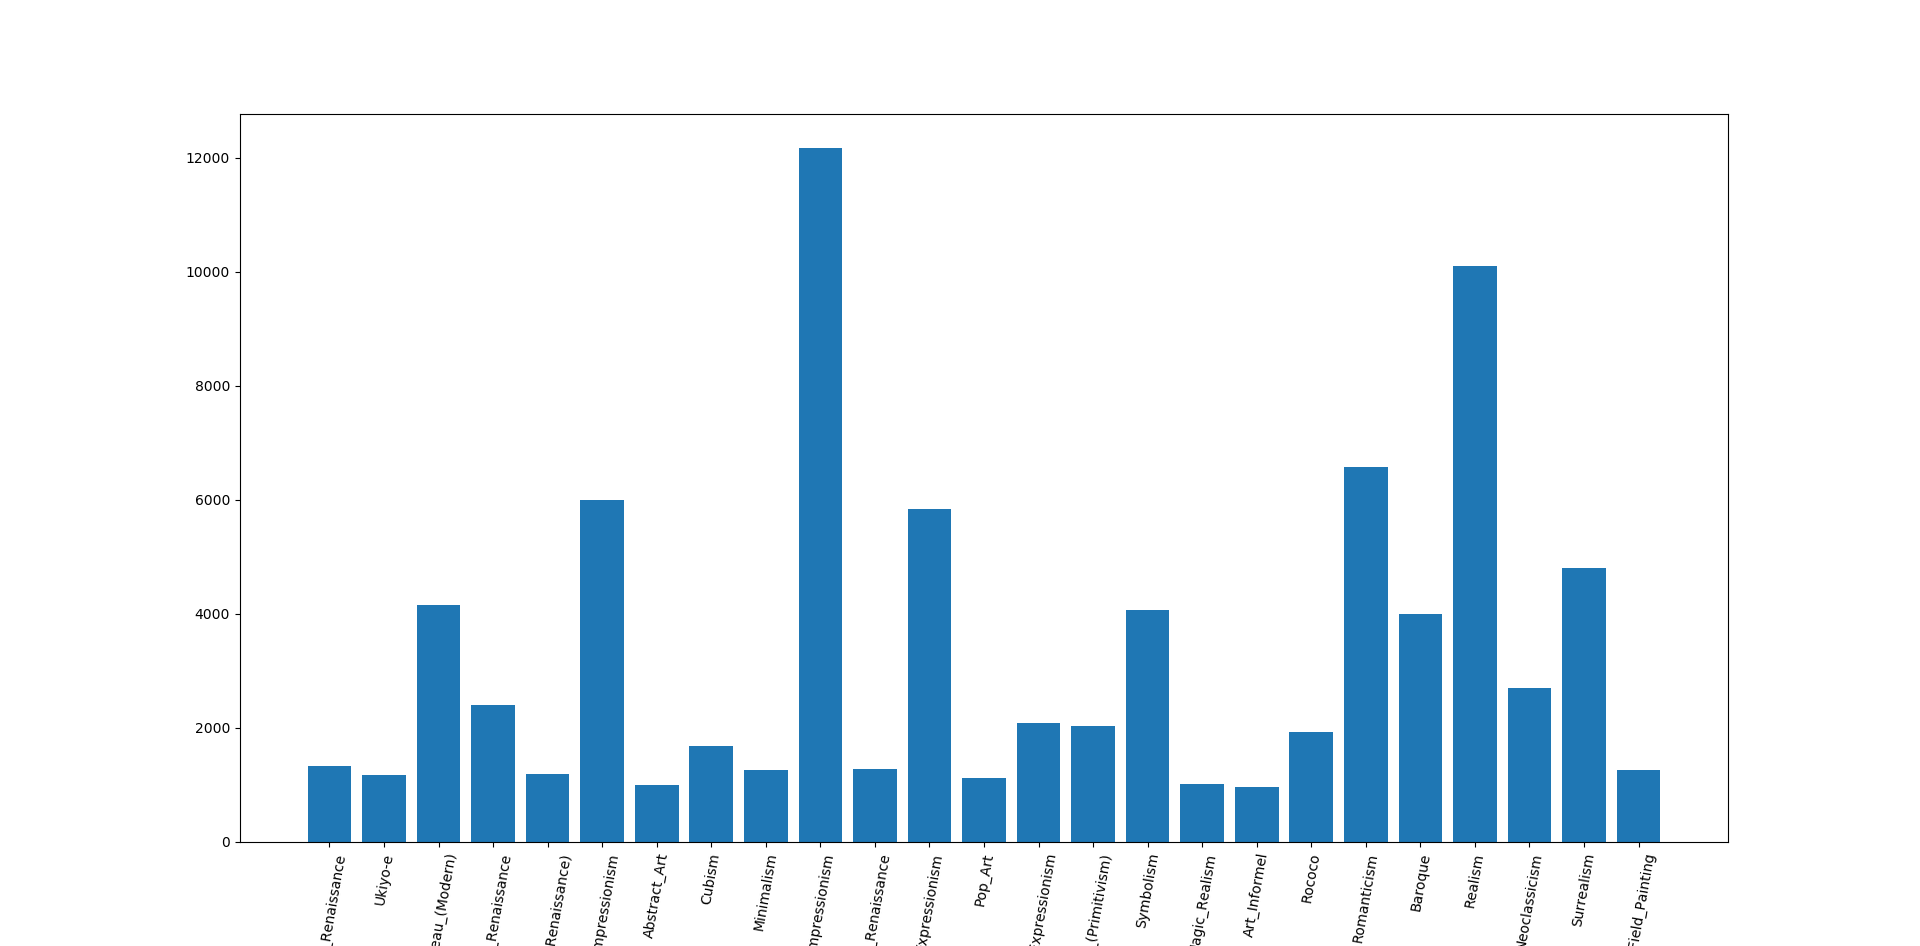
\includegraphics[scale = 0.3]{images/wp_distrib.png}
\end{figure}


After val train and test splitting : 
train = 66 574
test = 8 226
val = 7408

\subsection{Other database ?}